\scanpage{69}
\figure{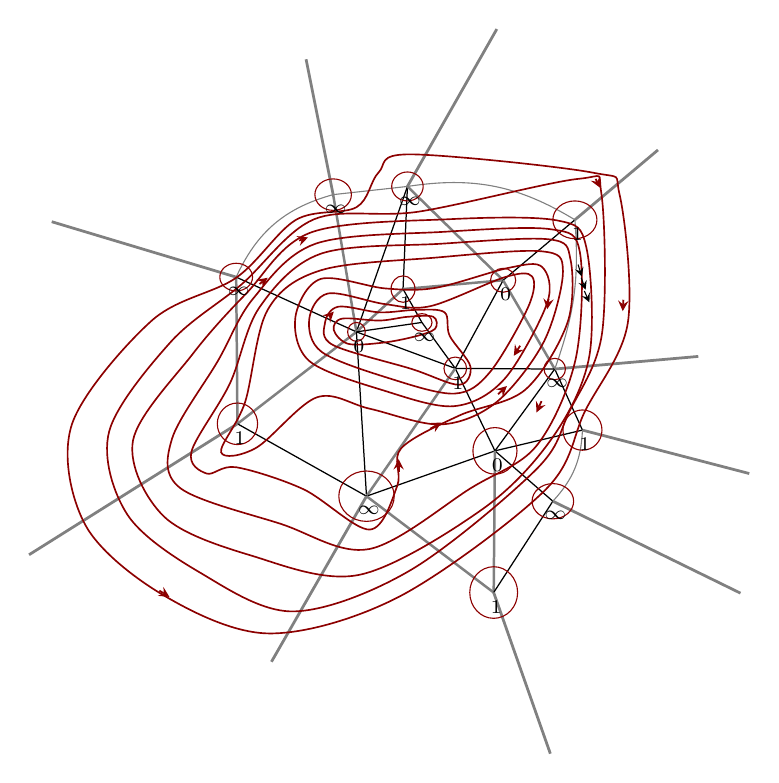
\begin{tikzpicture}[x=.008cm,y=-.008cm,>=stealth]
\coordinate (a) at (878,350);
\coordinate (b) at (996,337);
\coordinate (c) at (1262,390);
\coordinate (d) at (724,481);
\coordinate (e) at (989,500);
\coordinate (f) at (915,568);
\coordinate (g) at (1019,553);
\coordinate (h) at (1148,486);
\coordinate (i) at (1072,626);
\coordinate (j) at (1230,627);
\coordinate (k) at (726,714);
\coordinate (l) at (931,829);
\coordinate (m) at (1135,757);
\coordinate (n) at (1274,724);
\coordinate (o) at (1227,837);
\coordinate (p) at (1133,982);
\draw[gray,line width=.9pt] (f)--(a);
\draw[black,line width=.45pt] (f)--(b);
\draw[black,line width=.45pt] (f)--(d);
\draw[gray,line width=.9pt] (f)--(e);
\draw[black,line width=.45pt] (f)--(g);
\draw[black,line width=.45pt] (f)--(i);
\draw[gray,line width=.9pt] (f)--(k);
\draw[black,line width=.45pt] (f)--(l);
\draw[black,line width=.45pt] (b)--(e);
\draw[gray,line width=.9pt] (e)--(h);
\draw[black,line width=.45pt] (e)--(g);
\draw[black,line width=.45pt] (g)--(i);
\draw[gray,line width=.9pt] (b)--(h);
\draw[black,line width=.45pt] (c)--(h);
\draw[black,line width=.45pt] (h)--(i);
\draw[gray,line width=.9pt] (h)--(j);
\draw[black,line width=.45pt] (i)--(j);
\draw[black,line width=.45pt] (i)--(m);
\draw[gray,line width=.9pt] (i)--(l);
\draw[black,line width=.45pt] (j)--(m);
\draw[black,line width=.45pt] (j)--(n);
\draw[gray,line width=.9pt] (d)--(k);
\draw[black,line width=.45pt] (k)--(l);
\draw[black,line width=.45pt] (l)--(m);
\draw[gray,line width=.9pt] (l)--(p);
\draw[black,line width=.45pt] (m)--(n);
\draw[black,line width=.45pt] (m)--(o);
\draw[gray,line width=.9pt] (m)--(p);
\draw[black,line width=.45pt] (o)--(p);
\draw[gray] (a) to[bend right=25] (d);
\draw[gray] (a)--(b);
\draw[gray] (b) to[bend left=20] (c);
\draw[gray] (c) to[bend left=12] (j);
\draw[gray] (n) to[bend left=20] (o);
\draw[gray,line width=1pt] (a)--(835,135);
\draw[gray,line width=1pt] (b)--(1138,87);
\draw[gray,line width=1pt] (c)--(1394,279);
\draw[gray,line width=1pt] (d)--(431,393);
\draw[gray,line width=1pt] (j)--(1458,607);
\draw[gray,line width=1pt] (k)--(395,922);
\draw[gray,line width=1pt] (l)--(780,1092);
\draw[gray,line width=1pt] (n)--(1539,793);
\draw[gray,line width=1pt] (o)--(1525,983);
\draw[gray,line width=1pt] (p)--(1223,1238);
\draw[red!55!black,line width=.6pt] plot[smooth cycle,tension=.55] coordinates {(724,482) (590,550) (463,715) (484,874) (608,986) (777,1047) (984,988) (1215,819) (1278,694) (1346,554) (1333,350) (1290,315) (1000,286) (950,315) (915,370) (819,390)};
\draw[red!55!black,line width=.6pt] plot[smooth cycle,tension=.55] coordinates {(732,493) (620,584) (522,727) (551,858) (666,950) (814,1012) (1000,947) (1200,787) (1253,695) (1305,571) (1304,348) (1267,325) (1014,377) (848,389)};
\draw[red!55!black,line width=.6pt] plot[smooth cycle,tension=.55] coordinates {(740,507) (655,603) (560,741) (609,861) (747,923) (919,954) (1116,849) (1227,735) (1285,606) (1280,433) (1234,391) (1063,389) (843,410)};
\draw[red!55!black,line width=.6pt] plot[smooth cycle,tension=.55] coordinates {(751,515) (695,614) (622,738) (635,816) (795,873) (935,913) (1097,816) (1201,749) (1263,612) (1270,442) (1224,405) (1055,409) (850,428)};
\draw[red!55!black,line width=.6pt] plot[smooth cycle,tension=.55] coordinates {(761,529) (714,650) (653,758) (677,793) (724,783) (831,818) (936,882) (980,812) (986,753) (1078,701) (1183,660) (1250,554) (1255,453) (1221,421) (1049,428) (858,444)};
\draw[red!55!black,line width=.6pt] plot[smooth cycle,tension=.55] coordinates {(774,533) (738,680) (700,759) (756,752) (852,672) (936,690) (1049,715) (1137,680) (1213,583) (1243,471) (1209,440) (1041,450) (859,470)};
\draw[red!55!black,line width=.6pt] plot[smooth cycle,tension=.55] coordinates {(858,484) (818,545) (841,615) (958,661) (1070,686) (1150,643) (1218,522) (1210,465) (1158,466) (1041,498) (961,499)};
\draw[red!55!black,line width=.6pt] plot[smooth cycle,tension=.55] coordinates {(870,507) (840,548) (860,600) (968,642) (1071,666) (1127,632) (1188,528) (1194,480) (1151,481) (1033,527) (961,524)};
\draw[red!55!black,line width=.6pt] plot[smooth cycle,tension=.55] coordinates {(886,528) (865,554) (878,589) (1003,627) (1078,652) (1096,623) (1063,574) (1055,537) (1010,533) (952,537)};
\draw[red!55!black,line width=.6pt] plot[smooth cycle,tension=.55] coordinates {(892,547) (879,565) (902,587) (958,585) (1009,575) (1040,563) (1037,544) (997,544) (952,550)};
\draw[red!55!black] (a) ellipse (29 and 25);
\draw[red!55!black] (b) ellipse (25 and 23);
\draw[red!55!black] (c) ellipse (35 and 30);
\draw[red!55!black] (d) ellipse (26 and 22);
\draw[red!55!black] (e) ellipse (19 and 21);
\draw[red!55!black] (f) ellipse (14 and 15);
\draw[red!55!black] (g) ellipse (16 and 14);
\draw[red!55!black] (h) ellipse (20 and 19);
\draw[red!55!black] (i) ellipse (18 and 18);
\draw[red!55!black] (j) ellipse (17 and 17);
\draw[red!55!black] (k) ellipse (32 and 33);
\draw[red!55!black] (l) ellipse (44 and 40);
\draw[red!55!black] (m) ellipse (35 and 37);
\draw[red!55!black] (n) ellipse (31 and 32);
\draw[red!55!black] (o) ellipse (33 and 28);
\draw[red!55!black] (p) ellipse (38 and 41);
\node[font=\scriptsize,inner sep=0pt] at (882,373) {$\unsure{\infty}$};
\node[font=\scriptsize,inner sep=0pt] at (1000,360) {$\unsure{\infty}$};
\node[font=\scriptsize,inner sep=0pt] at (1266,413) {$1$};
\node[font=\scriptsize,inner sep=0pt] at (728,504) {$\unsure{\infty}$};
\node[font=\scriptsize,inner sep=0pt] at (993,523) {$\unsure{1}$};
\node[font=\scriptsize,inner sep=0pt] at (919,591) {$0$};
\node[font=\scriptsize,inner sep=0pt] at (1023,576) {$\infty$};
\node[font=\scriptsize,inner sep=0pt] at (1152,509) {$0$};
\node[font=\scriptsize,inner sep=0pt] at (1076,649) {$1$};
\node[font=\scriptsize,inner sep=0pt] at (1234,650) {$\infty$};
\node[font=\scriptsize,inner sep=0pt] at (730,737) {$1$};
\node[font=\scriptsize,inner sep=0pt] at (935,852) {$\infty$};
\node[font=\scriptsize,inner sep=0pt] at (1139,780) {$0$};
\node[font=\scriptsize,inner sep=0pt] at (1278,747) {$1$};
\node[font=\scriptsize,inner sep=0pt] at (1231,860) {$\infty$};
\node[font=\scriptsize,inner sep=0pt] at (1137,1005) {$1$};
\draw[->,red!55!black,line width=.65pt] (602,979)--(618,989);
\draw[->,red!55!black,line width=.65pt] (1295,325)--(1302,339);
\draw[->,red!55!black,line width=.65pt] (1339,517)--(1338,535);
\draw[->,red!55!black,line width=.65pt] (1209,678)--(1201,696);
\draw[->,red!55!black,line width=.65pt] (982,791)--(982,770);
\draw[->,red!55!black,line width=.65pt] (1032,722)--(1050,712);
\draw[->,red!55!black,line width=.65pt] (873,542)--(879,536);
\draw[->,red!55!black,line width=.65pt] (761,492)--(774,482);
\draw[->,red!55!black,line width=.65pt] (824,423)--(838,418);
\draw[->,red!55!black,line width=.65pt] (1175,590)--(1165,606);
\draw[->,red!55!black,line width=.65pt] (1220,516)--(1218,532);
\draw[->,red!55!black,line width=.65pt] (1140,667)--(1154,654);
\draw[->,black] (1272,482)--(1279,501);
\draw[->,black] (1277,503)--(1285,521);
\draw[->,black] (1267,461)--(1273,480);
\end{tikzpicture}}
% crop-candidate: scan 69


\mspage{68}
